\documentclass[11pt]{article}

% ---------- Packages ----------
\usepackage[utf8]{inputenc}
\usepackage[T1]{fontenc}
\usepackage[margin=2.5cm]{geometry}
\usepackage{cite}                 
\usepackage{graphicx}
\usepackage{amsmath,amssymb}
\usepackage{booktabs}
\usepackage{multirow}
\usepackage{array}
\usepackage{longtable}
\usepackage{xcolor}
\usepackage{tikz}
\usepackage{svg}
\usetikzlibrary{arrows.meta, positioning, fit, backgrounds, calc, decorations.pathreplacing, patterns}
\usepackage{pgfplots}
\pgfplotsset{compat=1.17}
\usepackage{caption}
\usepackage{hyperref}
\usepackage{enumitem}
\usepackage{fancyhdr}
\usepackage{titlesec}

\hypersetup{colorlinks=true, linkcolor=blue!50!black, citecolor=blue!50!black, urlcolor=blue!50!black}

\pagestyle{fancy}
\setlength{\headheight}{14pt}
\fancyhf{}
\fancyhead[L]{Extraction of Robust Commands from SSVEP Signals for Use in BCI}
\fancyhead[R]{\thepage}
\renewcommand{\headrulewidth}{0.4pt}

\titleformat{\section}{\normalfont\Large\bfseries}{\thesection}{1em}{}
\titleformat{\subsection}{\normalfont\large\bfseries}{\thesubsection}{1em}{}

\newcommand{\todocite}[1]{\textcolor{red}{\textbf{[ADDITIONAL SOURCE -- VERIFY: #1]}}}
\newcommand{\verifynote}[1]{\textcolor{orange!80!black}{\footnotesize [Verify: #1]}}
\newcommand{\todofill}[1]{\textcolor{red}{\textbf{[TO BE FILLED: #1]}}}

\title{\textbf{Extraction of Robust Commands from SSVEP Signals \\ for Use in Brain--Computer Interfaces} \\[0.3cm]
\large Literature Review, Proposed Robustness Mechanisms, and Prototype Validation}
\author{Farooq Danesh Amooz \\ Department of Electrical and Computer Engineering \\ University of Tabriz \\ \small Supervisor: Prof. Hadi Seyedarabi}
\date{\today}

\begin{document}

\maketitle

\begin{abstract}
\noindent
Steady-state visually evoked potential (SSVEP)-based brain--computer interfaces (BCIs) translate a user's gaze at a flickering visual target into a discrete command, without requiring muscular activity. Decoding methods have evolved from correlation-based statistics to deep neural networks, substantially improving accuracy and information transfer rate (ITR); however, this report argues that ``robustness'' in this field actually spans three distinct, unequally mature dimensions: within-trial noise robustness, cross-subject and low-calibration robustness, and adversarial robustness. Building on a review of approximately 20 papers, three concrete mechanisms are proposed to target these dimensions -- dual-modality color-plus-frequency redundancy on a safety-critical command (H1), trial-by-trial online adaptation (H2), and an alternative code-modulated (c-VEP) encoding (H3) -- implemented on a purpose-built five-key wheelchair control panel. A first single-subject hardware and software prototype validates the SSVEP decoding pipeline end to end, and produces a diagnosed, literature-consistent negative result: training-free c-VEP decoding fails on this hardware because it neglects the subject-specific temporal response function, independently reproducing the same calibration-robustness argument developed from the literature review. H1--H3 remain proposed and untested; synchronized, multi-condition data collection is identified as the project's immediate next step.
\end{abstract}

\vspace{0.3cm}
\noindent\textbf{\textit{Keywords}---}Brain--computer interface, steady-state visual evoked potential (SSVEP), code-modulated visual evoked potential (c-VEP), robustness, online adaptation, calibration, multimodal stimulus encoding.
\vspace{0.3cm}

\tableofcontents

\begin{figure}[htbp]
\centering
\includegraphics[width=\textwidth]{Robust_SSVEP_Command_Extraction_Workflow.png}
\caption{The report general infographics}
\label{fig:Report General Infographics}
\end{figure}

% =====================================================================
\section{Introduction}
% =====================================================================

\subsection{Brain--Computer Interfaces: Definition and Processing Pipeline}

A brain--computer interface (BCI) is a hardware and software system that translates neural activity directly into commands for an external device, bypassing the normal output pathways of the peripheral nervous system and muscles~\cite{nicolasalonso2012bci}. Nicolas-Alonso and Gomez-Gil's widely cited review decomposes a generic BCI into five sequential processing stages: (i) \textit{signal acquisition}, where a neuroimaging modality such as electroencephalography (EEG) records brain activity; (ii) \textit{preprocessing / signal enhancement}, where artifacts and background noise are attenuated; (iii) \textit{feature extraction}, where the informative components of the signal are isolated; (iv) \textit{classification}, where the extracted features are mapped to a discrete command; and (v) \textit{control interface}, where the recognized command drives an application (a speller, wheelchair, robotic arm, and so on)~\cite{nicolasalonso2012bci}. Figure~\ref{fig:pipeline} depicts this pipeline. It is a closed loop: the outcome observed by the user (for example, a letter appearing on a speller) can influence what the user attends to next. Hence, the control interface stage feeds back into signal acquisition.

\begin{figure}[htbp]
\centering
\resizebox{\textwidth}{!}{%
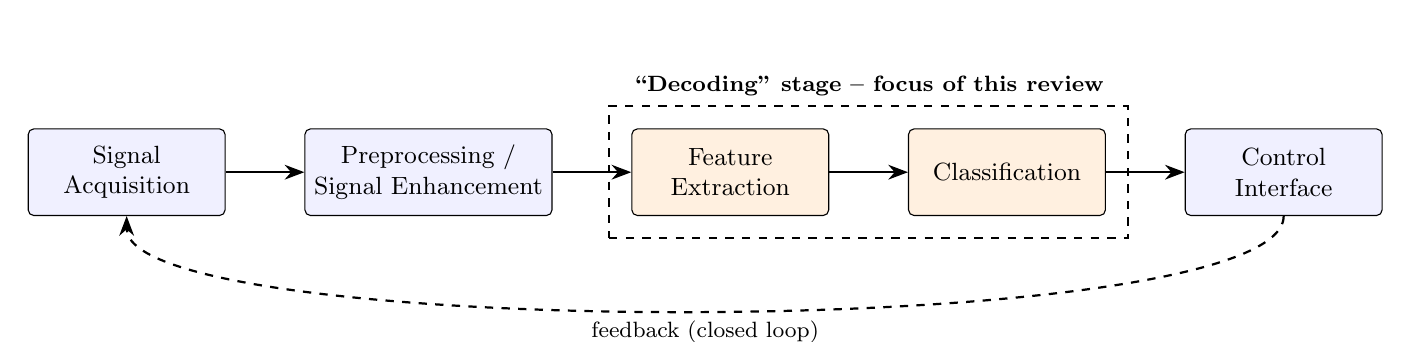
\begin{tikzpicture}[
  box/.style={draw, rounded corners=2pt, minimum height=1.1cm, minimum width=2.5cm, align=center, font=\small, fill=blue!6},
  decodebox/.style={draw, rounded corners=2pt, minimum height=1.1cm, minimum width=2.5cm, align=center, font=\small, fill=orange!12},
  arr/.style={-{Stealth[length=2.5mm]}, thick}
]
  \node[box] (acq)  {Signal\\Acquisition};
  \node[box, right=1.0cm of acq] (pre) {Preprocessing /\\Signal Enhancement};
  \node[decodebox, right=1.0cm of pre] (feat) {Feature\\Extraction};
  \node[decodebox, right=1.0cm of feat] (clas) {Classification};
  \node[box, right=1.0cm of clas] (ctrl) {Control\\Interface};

  \draw[arr] (acq) -- (pre);
  \draw[arr] (pre) -- (feat);
  \draw[arr] (feat) -- (clas);
  \draw[arr] (clas) -- (ctrl);

  \draw[arr, dashed] (ctrl.south) .. controls +(0,-1.6) and +(0,-1.6) .. (acq.south)
      node[midway, below, font=\footnotesize] {feedback (closed loop)};

  \begin{scope}[on background layer]
    \node[fit=(feat)(clas), draw, dashed, thick, inner sep=8pt, label={[font=\footnotesize]above:\textbf{``Decoding'' stage -- focus of this review}}] (decode) {};
  \end{scope}
\end{tikzpicture}
}
\caption{The five-stage BCI processing pipeline, redrawn from Nicolas-Alonso and Gomez-Gil~\cite{nicolasalonso2012bci}. For SSVEP-BCIs, feature extraction and classification are frequently performed by a single algorithm (e.g.\ CCA directly outputs a class label), so this review treats them jointly as the ``decoding'' stage.}
\label{fig:pipeline}
\end{figure}

Among the neural signals used to drive this pipeline, EEG is the dominant choice because it is non-invasive, inexpensive, portable, and has millisecond-scale temporal resolution~\cite{nicolasalonso2012bci}. Within EEG-based BCI paradigms, the steady-state visually evoked potential (SSVEP) is one of the most widely used control signals, alongside the P300 event-related potential and motor imagery~\cite{nicolasalonso2012bci}.

\subsection{The SSVEP Paradigm}

An SSVEP is a periodic electrical response of the visual cortex that is evoked when a subject fixates on a visual stimulus flickering at a fixed frequency (typically greater than roughly 4--6~Hz); the resulting EEG signal, recorded over the occipital region, oscillates at the same frequency as the stimulus and at its harmonics~\cite{vialatte2010ssvep}. Vialatte \textit{et al.}'s review of 40 years of SSVEP research in cognitive and clinical neuroscience situates SSVEP-BCI as one of several application domains for this signal, alongside its long-standing use in the study of visual attention, binocular rivalry, and clinical assessment of the visual pathway~\cite{vialatte2010ssvep}.

An SSVEP-BCI exploits this response as follows: several visual targets are presented simultaneously, each flickering at a distinct frequency (and, in more recent paradigms, also at a distinct phase); the user looks at the target corresponding to the command he or she wishes to issue; and the decoding stage identifies which frequency (and phase) is present in the recorded EEG, thereby recovering the intended command~\cite{lin2007cca}. Because the mapping from a fixed stimulus set to a fixed frequency set is known in advance, SSVEP-BCI is fundamentally a \emph{frequency-recognition} problem, and essentially all of the methods reviewed in Section~2 can be understood as different strategies for estimating, from a short segment of multichannel EEG, which candidate frequency (and, where used, phase or code) the signal is most consistent with.

SSVEP-BCI is attractive relative to other EEG paradigms for three reasons that recur throughout the literature reviewed below: a comparatively high signal-to-noise ratio (SNR) at the occipital electrodes, a high achievable information transfer rate (ITR, the standard combined speed-and-accuracy metric for BCI communication, expressed in bits per minute), and a low requirement for extensive user training relative to motor-imagery BCIs~\cite{li2024sutl}.

\subsection{Problem Statement: What Does ``Robust'' Command Generation Mean?}

The assigned topic of this report, \emph{extraction of robust commands from SSVEP signals}, requires a precise definition of robustness, because the term is used in the literature to describe at least three distinct properties of a decoding algorithm, which are not automatically related to one another:

\begin{enumerate}[label=(\alph*)]
  \item \textbf{Robustness to within-trial noise and short data length.} Given a fixed subject and a fixed EEG channel set, how much recording time is required before the decoder can reliably separate the target frequency from background EEG activity and from the other candidate frequencies? This is the sense of ``robustness'' addressed by the classical spatial-filtering literature (CCA, MSI, FBCCA, TRCA), reviewed in Section~2.2.

  \item \textbf{Robustness across subjects and across amounts of calibration data.} EEG signals are known to vary substantially between individuals~\cite{zerafa2018train}. A decoder that performs well for the subjects it was calibrated on may perform poorly for a new subject with no calibration data at all, or may even suffer \emph{negative transfer}, in which using another subject's data actively degrades performance relative to a training-free baseline~\cite{li2024sutl}. This sense of robustness also has a within-subject counterpart, relevant later in this report: a decoder calibrated once, at the start of a session, may drift out of alignment with the same subject's own brain signals as the session continues, because EEG is non-stationary~\cite{nicolasalonso2012bci}.

  \item \textbf{Robustness to deliberately adversarial input.} A decoder that is accurate and calibration-efficient may still be vulnerable to a malicious actor who injects a crafted perturbation into the EEG signal to force a specific, attacker-chosen output~\cite{bian2022squarewave}. This is a comparatively new and comparatively under-studied sense of robustness, discussed in Section~3.3.
\end{enumerate}

This report's working position, developed further in Section~3, is that dimension (a) has been substantially, though not completely, addressed by the methodological line CCA~$\rightarrow$~FBCCA~$\rightarrow$~TRCA, whereas dimension (b) remains an active bottleneck at both the cross-subject and the within-subject (temporal drift) level, and dimension (c) remains largely unexplored outside a single paper in the reviewed set. Sections~4--5 identify three specific, testable mechanisms -- targeting dimensions (a), (b), and (c) respectively -- and Sections~6--7 describe a first hardware prototype and single-subject pilot built to test them.

\subsection{Organization of This Report}

Section~2.1 introduces the organizing framework used throughout the review: the five-stage BCI pipeline of Figure~\ref{fig:pipeline}, combined with Zerafa \textit{et al.}'s three-way taxonomy of decoding methods by their training requirement (training-free, subject-specific, subject-independent)~\cite{zerafa2018train}. Section~2.2 surveys the state of the art within each resulting category, drawing on ten core papers and several additional papers published in 2024--2026. Section~3 uses the same taxonomy to argue that ``robustness'' spans three distinct dimensions. Section~4 explains why three specific mechanisms (H1, H2, H3) are expected to improve robustness along these dimensions. Section~5 details the experimental protocol designed to test H1--H3. Section~6 describes the physical stimulus panel built for this project. Section~7 reports a first, single-subject prototype data-collection and analysis pass. Section~8 summarizes what has been accomplished and what remains. Section~9 concludes.

% =====================================================================
\section{Related Work: SSVEP Decoding Methods}
% =====================================================================

\subsection{Organizing Framework: Pipeline Stage $\times$ Training Taxonomy}
\label{sec:framework}

\subsubsection{Zerafa et al.'s training-requirement taxonomy}

Zerafa \textit{et al.}~\cite{zerafa2018train} surveyed the SSVEP feature-extraction literature and sorted every reviewed method into exactly one of three categories, based on what calibration data, if any, it requires from the end user before it can be used:

\begin{itemize}
  \item \textbf{Training-free} (also called calibration-free or unsupervised): the method works immediately for a new user, with no calibration recording of any kind. Canonical correlation analysis (CCA) is the standard example.
  \item \textbf{Subject-specific} (also called calibration-based or supervised): the method requires calibration data recorded from the specific end user before it can be used for that user.
  \item \textbf{Subject-independent}: the method requires calibration data, but that data is drawn from a pool of \emph{other} subjects; the end user performs zero calibration.
\end{itemize}

Zerafa \textit{et al.} report that, across the studies they surveyed, training-free methods showed systematically lower accuracy and ITR than both subject-specific and subject-independent methods, with gaps in the reported ranges of roughly 7--41 percentage points of accuracy and 17--65\% of ITR relative to subject-specific methods, and roughly 19--46 percentage points of accuracy and 28--63\% of ITR relative to subject-independent methods~\cite{zerafa2018train}. The authors are explicit, however, that these ranges are pooled across different studies with different experimental conditions (stimulus count, trial length, electrode montage) rather than the output of one controlled comparison, and that ``large variations in the performances of the same method across different studies'' make any single number unreliable as an absolute benchmark~\cite{zerafa2018train}. This taxonomy is adopted here as the primary organizing tool for the literature review, both because it is the framework used by a dedicated survey paper on the training-requirement question, and because -- as argued in Section~3 -- the gap it identifies between training-free and calibration-based methods is a direct entry point for the mechanisms proposed in Section~4.

\subsubsection{Where the taxonomy applies within the pipeline}

The training-requirement taxonomy is a property of the \emph{decoding algorithm}, i.e.\ of the feature-extraction and classification stages in Figure~\ref{fig:pipeline}. It says nothing, by itself, about the earlier signal-acquisition and preprocessing stages, nor about the downstream control-interface stage, which are largely determined by hardware and application choices rather than by the calibration strategy of the decoder. Table~\ref{tab:pipeline-taxonomy} makes this scope explicit by crossing all five pipeline stages with the three taxonomy categories, rather than assuming, without checking, that the taxonomy is relevant everywhere.

\begin{table}[htbp]
\centering
\caption{Pipeline stage $\times$ training-taxonomy matrix. Cells give representative methods from the reviewed paper set; ``--'' marks a stage at which the training taxonomy does not meaningfully apply.}
\label{tab:pipeline-taxonomy}
\small
\resizebox{\textwidth}{!}{%
\begin{tabular}{@{}p{2.6cm} p{4.6cm} p{5.4cm} p{4.6cm}@{}}
\toprule
\textbf{Pipeline stage} & \textbf{Training-free} & \textbf{Subject-specific} & \textbf{Subject-independent} \\
\midrule
Signal acquisition & \multicolumn{3}{p{14.6cm}}{-- (electrode montage, sampling rate, and stimulus hardware are chosen independently of the decoder's calibration requirement)} \\
\addlinespace
Preprocessing & \multicolumn{3}{p{14.6cm}}{-- (band-pass / notch filtering and artifact rejection are applied uniformly, before any subject-specific or pooled data enters the model)} \\
\addlinespace
Feature extraction \& classification (``decoding'') &
CCA~\cite{lin2007cca}, MSI~\cite{zhang2014msi}, FBCCA~\cite{chen2015fbcca}, JFPM~\cite{chen2015pnas} &
TRCA / eTRCA~\cite{nakanishi2018trca}, eTRCA+sbCNN~\cite{wei2025etrcasbcnn}, t-SSVEPformer+JFPTS~\cite{ding2026jfpts}, TDCA~\cite{liu2021tdca}, EEGNet (per-subject fine-tuning)~\cite{lawhern2018eegnet} &
SUTL~\cite{li2024sutl} and the transfer-learning / domain-alignment methods surveyed by Zhang and Tao~\cite{zhang2026mobilereview} \\
\addlinespace
Control interface/application & \multicolumn{3}{p{14.6cm}}{-- (a speller, wheelchair-control, or drone-control application layer can, in principle, sit on top of any decoder in the two columns to the left)} \\
\bottomrule
\end{tabular}
}
\end{table}

Two consequences of Table~\ref{tab:pipeline-taxonomy} are used repeatedly in the rest of this review. First, because feature extraction and classification are usually fused into a single algorithmic step for SSVEP decoding (a correlation or synchronization score is computed and directly arg-maxed into a class label, without a separately trained classifier stage), this report follows the convention, already used informally in Section~1, of referring to that fused stage simply as ``decoding.'' Second, the taxonomy gives a natural axis along which to organize Section~2.2: within the decoding stage, methods are grouped first by whether they are classical (hand-designed correlation or spatial-filtering statistics) or based on deep learning, and second by their position in the training-free / subject-specific / subject-independent taxonomy.

\subsection{State of the Art by Category}
\label{sec:sota}

Figure~\ref{fig:timeline} gives a chronological overview of the reviewed decoding methods, color-coded by taxonomy category, before the category-by-category discussion below.

\begin{figure}[htbp]
\centering
\resizebox{\textwidth}{!}{%
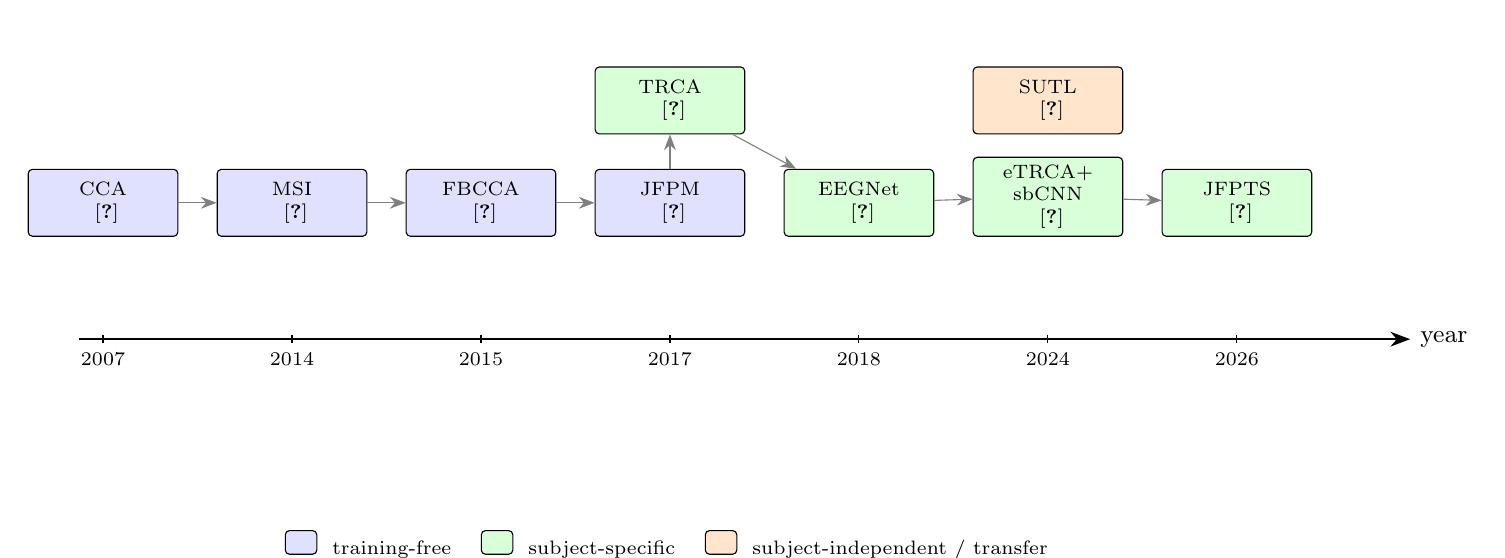
\begin{tikzpicture}[
  node distance=1.3cm and 0.35cm,
  every node/.style={font=\scriptsize},
  ev/.style={draw, rounded corners=1.5pt, align=center, minimum width=1.9cm, minimum height=0.85cm, inner sep=3pt}
]
  \draw[thick, -{Stealth[length=2.5mm]}] (-0.3,0) -- (16.6,0) node[right, font=\small] {year};

  \foreach \x/\yr in {0/2007, 2.4/2014, 4.8/2015, 7.2/2017, 9.6/2018, 12.0/2024, 14.4/2026}
    \draw (\x,0.05) -- (\x,-0.05) node[below, font=\scriptsize] {\yr};

  \node[ev, fill=blue!12, above=of {(0,0)}]  (cca) {CCA \\ \cite{lin2007cca}};
  \node[ev, fill=blue!12, above=of {(2.4,0)}] (msi) {MSI \\ \cite{zhang2014msi}};
  \node[ev, fill=blue!12, above=of {(4.8,0)}] (fbcca) {FBCCA \\ \cite{chen2015fbcca}};
  \node[ev, fill=blue!12, above=of {(7.2,0)}] (jfpm) {JFPM \\ \cite{chen2015pnas}};
  \node[ev, fill=green!15, above=of {(7.2,0)}, yshift=1.3cm] (trca) {TRCA \\ \cite{nakanishi2018trca}};
  \node[ev, fill=green!15, above=of {(9.6,0)}] (eegnet) {EEGNet \\ \cite{lawhern2018eegnet}};
  \node[ev, fill=green!15, above=of {(12.0,0)}] (hyb) {eTRCA+ \\ sbCNN \\ \cite{wei2025etrcasbcnn}};
  \node[ev, fill=orange!20, above=of {(12.0,0)}, yshift=1.3cm] (sutl) {SUTL \\ \cite{li2024sutl}};
  \node[ev, fill=green!15, above=of {(14.4,0)}] (jfpts) {JFPTS \\ \cite{ding2026jfpts}};

  \foreach \a/\b in {cca/msi, msi/fbcca, fbcca/jfpm, jfpm/trca, trca/eegnet, eegnet/hyb, hyb/jfpts}
    \draw[-{Stealth[length=2mm]}, gray] (\a) -- (\b);

  \node[below=2.3cm of {(7.2,0)}, align=left, font=\scriptsize] (legend) {
    \tikz\node[ev, fill=blue!12, minimum width=0.4cm, minimum height=0.3cm]{}; ~training-free \quad
    \tikz\node[ev, fill=green!15, minimum width=0.4cm, minimum height=0.3cm]{}; ~subject-specific \quad
    \tikz\node[ev, fill=orange!20, minimum width=0.4cm, minimum height=0.3cm]{}; ~subject-independent / transfer
  };
\end{tikzpicture}
}
\caption{Chronological overview of the reviewed decoding methods, color-coded by training-taxonomy category. Placement is approximate and intended to show methodological lineage, not precise publication months.}
\label{fig:timeline}
\end{figure}

\subsubsection{Training-free correlation-based methods}

\textbf{CCA.} Lin \textit{et al.} introduced canonical correlation analysis to SSVEP frequency recognition, computing, for each candidate frequency, the maximal correlation between a linear combination of the multichannel EEG and a linear combination of sine/cosine reference signals at that frequency, and selecting the frequency with the highest correlation~\cite{lin2007cca}. They also identified an optimal eight-channel bipolar electrode configuration for maximizing SNR and showed that CCA outperformed the previously standard power spectral density analysis (PSDA) approach for most subjects~\cite{lin2007cca}. The authors themselves note two limitations that recur in later work: only the single largest CCA coefficient is used for the decision, discarding potentially useful subordinate correlations, and the method assumes an essentially linear relationship between the reference signals and the EEG, whereas the visual pathway is known to be non-linear~\cite{lin2007cca}.

\textbf{MSI.} Zhang \textit{et al.} proposed the multivariate synchronization index (MSI), which replaces CCA's correlation coefficient with an entropy-based synchronization measure (the S-estimator, bounded between 0 and 1) computed between the multichannel EEG and the same sine/cosine references used by CCA~\cite{zhang2014msi}. In simulation at SNR levels from $-7$ to $-20$~dB and in an 11-subject offline data set, MSI consistently outperformed both CCA and the minimum energy combination (MEC) method, with its advantage largest specifically at short data lengths (1~s) and few channels (4)~\cite{zhang2014msi}. In an online robot-control test with 10 subjects and 4 targets, MSI achieved 86\%~$\pm$~13.08\% accuracy and 19.43~$\pm$~8.16 bits/min ITR~\cite{zhang2014msi}; the authors attribute the comparatively modest ITR mainly to the small number of targets used, not to a weakness of MSI itself~\cite{zhang2014msi}. They also report that individual differences were large -- one subject scored 100\% while another scored only 60\% -- meaning MSI reduces, but does not eliminate, the practical need for subject-specific tuning~\cite{zhang2014msi}.

\textbf{FBCCA.} Chen \textit{et al.} observed that a naive attempt to extend CCA's reference signals with SSVEP harmonics had previously failed to improve performance, and proposed instead a filter-bank architecture (FBCCA) that splits the EEG into several sub-bands, runs CCA independently on each sub-band, and combines the sub-band correlations with weights that favor the lower, stronger sub-bands~\cite{chen2015fbcca}. Of three filter-bank designs tested, the one in which every sub-band starts at a harmonic frequency but extends to the top of the analyzed range (their design ``M3'') performed best, reaching 89.47\% accuracy and 145.52~bits/min offline, and 91.95\%~$\pm$~7.22\% accuracy and 151.18~$\pm$~20.34~bits/min ITR in a 10-subject online spelling test at a spelling rate of 33.3 characters per minute~\cite{chen2015fbcca}. As a training-free method, FBCCA is markedly faster to deploy than calibration-based alternatives, but the authors explicitly acknowledge that individually calibrated methods can still exceed its accuracy (they cite a 97\% vs.\ 92\% comparison against an extended-CCA calibration-based method), at the cost of a calibration session~\cite{chen2015fbcca}.

\textbf{JFPM.} Chen \textit{et al.}'s high-speed speller does not introduce a new correlation statistic, but a new stimulus-coding scheme: joint frequency-phase modulation (JFPM), in which each of 40 targets is assigned a unique combination of frequency \emph{and} phase, rather than frequency alone~\cite{chen2015pnas}. Because the added phase dimension helps separate closely spaced targets, JFPM allows a much shorter data window (0.5~s, versus the roughly 5~s required for frequency-only coding at the same spacing) while retaining classification accuracy~\cite{chen2015pnas}. The best grid-searched configuration reached 88.92\% offline accuracy and 4.32~bits/s; online cued spelling reached 91.04\%~$\pm$~6.73\% accuracy and 4.45~$\pm$~0.58~bits/s, which converts to approximately 267~bits/min~\cite{chen2015pnas}. The method's robustness claim rests on the finding that the brain's visual response latency is highly stable across trials (reported standard deviation on the order of a few milliseconds); the authors themselves flag this stability result as coming from supplementary material~\cite{chen2015pnas}.

\subsubsection{Subject-specific spatial filtering and deep learning}

\textbf{TRCA.} Nakanishi \textit{et al.} proposed task-related component analysis (TRCA), a subject-specific spatial filter obtained by solving an eigenvalue problem that maximizes the reproducibility of the EEG response across repeated trials of the same target~\cite{nakanishi2018trca}. Its ensemble extension, ensemble TRCA (eTRCA), combines the spatial filters learned for all 40 targets into a single filter bank. In an online cue-guided 40-target speller, ensemble TRCA reached 89.83\%~$\pm$~6.07\% accuracy and 325.33~$\pm$~38.17~bits/min ITR, using a spelling rate of 0.8~s per character~\cite{nakanishi2018trca}; the authors reported this as the highest ITR published for an EEG-based BCI at the time. A free-spelling (uncued) variant reached 198.67~$\pm$~50.48~bits/min~\cite{nakanishi2018trca}. As a subject-specific method, TRCA's headline speed depends on a calibration session per user, and the authors note that their high spelling speed was demonstrated with experienced users; naive users would likely require a longer gaze-shifting interval~\cite{nakanishi2018trca}.

\textbf{TDCA.} Liu \textit{et al.} proposed task-discriminant component analysis (TDCA), a spatial-filtering method closely related to TRCA but designed to produce a single, class-generic spatial filter (rather than one filter per class), by maximizing the between-class scatter of the calibration data relative to its within-class scatter~\cite{liu2021tdca}. Because the resulting filter is generic rather than target-specific, it can, in principle, be reused across different stimulus sequences and layouts, which later work (Section~2.2.3 and Section~4.3) exploits to reduce the calibration burden of both SSVEP and c-VEP decoding~\cite{liu2021tdca}.

\textbf{EEGNet.} Lawhern \textit{et al.}'s EEGNet is a compact convolutional neural network built from depthwise and separable convolutions, designed to generalize across several different EEG-BCI paradigms (P300, error-related negativity, movement-related cortical potentials, and sensorimotor rhythms) rather than being specialized for SSVEP frequency recognition~\cite{lawhern2018eegnet}. It matched or outperformed larger reference CNN architectures within-subject, though a traditional Riemannian-geometry pipeline outperformed all tested CNNs, including EEGNet, in one cross-subject condition -- a result the authors report openly as a failure case rather than omitting it~\cite{lawhern2018eegnet}. Because EEGNet was not benchmarked head-to-head against CCA/FBCCA/TRCA on a shared SSVEP accuracy/ITR metric in the original paper, it is included in this review primarily for architectural reasons: its learned depthwise spatial filter is a data-driven counterpart to the hand-designed spatial filters of TRCA, TDCA, and CCA, and this structural parallel is used by several later SSVEP-specific deep networks (see below).

\textbf{eTRCA+sbCNN.} Wei \textit{et al.} propose a hybrid classification framework that trains eTRCA and a sub-band convolutional neural network (sbCNN) separately and then sums their classification score vectors, taking the frequency with the highest combined score~\cite{wei2025etrcasbcnn}. On the Benchmark and BETA public data sets, the combined model significantly outperformed either component model alone at almost every tested data length, channel count, and number of training trials, reaching a peak ITR of 249.47~bits/min (Benchmark) and 188.55~bits/min (BETA) at a 0.4~s data length~\cite{wei2025etrcasbcnn}. At a 1.0~s data length on the BETA data set, the combined model reached 84.88\% accuracy and 159.96~bits/min, compared with 72.89\% and 121.85~bits/min for TRCA alone and 59.37\% and 88.00~bits/min for FBCCA~\cite{wei2025etrcasbcnn}. The authors report one clear limitation: with only 3 EEG channels, or with only 0.2~s of data, eTRCA's own accuracy collapses, and the hybrid model's advantage over sbCNN alone disappears in those specific conditions~\cite{wei2025etrcasbcnn}.

\textbf{t-SSVEPformer + JFPTS.} Ding \textit{et al.} argue that existing deep-learning training strategies for SSVEP exploit either the frequency or the phase structure of the signal, but not both, and propose a two-stage joint frequency-phase training strategy (JFPTS): a first stage that samples training windows to emphasize frequency-component coverage, followed by a second, phase-locked stage that enforces consistent phase alignment within each target category~\cite{ding2026jfpts}. Applied to a transformer-based backbone (t-SSVEPformer), JFPTS reached a peak ITR of 264.37~$\pm$~14.56~bits/min on the Benchmark data set and 201.92~$\pm$~10.46~bits/min on BETA, both at a 0.3~s data length, exceeding the strong template-matching baselines TDCA and TRCA by 15--48~bits/min depending on data set~\cite{ding2026jfpts}. An ablation study confirmed that both stages of JFPTS contribute: at 0.3~s, JFPTS reached 76.83\%~$\pm$~3.04\% (Benchmark) and 64.71\%~$\pm$~2.30\% (BETA) accuracy, versus 63.25\%~$\pm$~3.19\% and 60.03\%~$\pm$~2.33\% for the frequency-only stage alone, and 45.96\%~$\pm$~3.95\% and 28.21\%~$\pm$~2.01\% for the phase-only stage alone~\cite{ding2026jfpts}. This paper was published in January 2026, after this reviewer's assigned reading list was first compiled, and is therefore also the most recent method covered in this report.

\subsubsection{Subject-independent and cross-subject transfer methods}

\textbf{SUTL.} Motivated explicitly by the calibration burden of subject-specific methods, Li \textit{et al.} propose an unsupervised cross-subject transfer-learning framework (SUTL) that combines a subject transferability estimation (STE) step, which screens which source subjects are actually useful for a given new (target) subject, with a multi-domain alignment step that makes the EEG distributions of different subjects more similar before transferring both generalization and subject-specific knowledge~\cite{li2024sutl}. On the Benchmark and BETA data sets, averaged across all tested signal lengths, SUTL reached 75.53\%~$\pm$~12.72\% accuracy (Benchmark) and 68.18\%~$\pm$~14.82\% accuracy (BETA), compared with 58.90\%~$\pm$~14.51\% and 54.65\%~$\pm$~15.19\% for the training-free FBCCA baseline, and 65--66\% for two other transfer baselines (CSSFT and tt-CCA)~\cite{li2024sutl}. Critically, the authors also show that a naive transfer baseline (tt-CCA) suffered from data-distribution mismatch on the BETA data set and exhibited \emph{negative transfer}, performing worse than the training-free FBCCA baseline it was supposed to improve on -- a direct empirical demonstration of the risk that motivates SUTL's subject-selection step~\cite{li2024sutl}.

\textbf{Deep-learning-for-mobile-BCI review.} Zhang and Tao's 2026 narrative review synthesizes post-2023 deep-learning SSVEP decoding work around three engineering-oriented themes: lightweight model architectures (for example, a calibration-free model compressed to 0.23~MB, and a transfer-learning method whose trainable weights are only 0.013\% of a non-transfer model~\cite{zhang2026mobilereview}), ultra-short time-window decoding, and cross-subject transfer and low-calibration strategies~\cite{zhang2026mobilereview}. The authors group cross-subject approaches into source-target knowledge mapping / instance transfer, domain-invariant representation learning with unsupervised distribution alignment (the same general family as SUTL), and physiologically inspired data augmentation~\cite{zhang2026mobilereview}. They explicitly flag, as a limitation of the field rather than of any single paper, that studies rarely report complete cross-subject generalization curves under a shared evaluation protocol, which makes rigorous quantitative comparison across cross-subject methods difficult~\cite{zhang2026mobilereview}.

\textbf{Online adaptation.} A complementary strategy to cross-subject transfer, but targeting the \emph{within}-subject side of dimension (b), is online adaptation: rather than collecting more data from other people, the decoder updates its own subject-specific template using the current user's own trials as a session continues. Wong \textit{et al.} show that this strategy measurably improves SSVEP-BCI performance relative to a static, once-calibrated classifier~\cite{wong2022onlineadaptation}. This paper is the direct methodological ancestor of the H2 mechanism proposed in Section~4.2.

\subsubsection{Code-modulated visual evoked potentials (c-VEP): an alternative encoding}

A separate design choice, orthogonal to the training-taxonomy axis above, is \emph{how} the visual stimulus itself is encoded. Instead of a fixed flicker frequency, a code-modulated visual evoked potential (c-VEP) stimulus flickers according to a pseudorandom binary sequence, with different targets typically distinguished by different time-shifts of a shared code~\cite{martinezcagigal2021cvepreview}. Early work established the online feasibility of correlation-based SSVEP/c-VEP decoding~\cite{bin2009online}; more recent work has focused specifically on reducing the calibration burden that c-VEP historically required. Thielen \textit{et al.} moved from full per-subject calibration toward zero-training c-VEP decoding~\cite{thielen2021zerotraining}; Miao \textit{et al.} introduced a one-minute single-target calibration stage combined with either a linear stimulus-response model or cross-subject transfer learning, reaching an information transfer rate of up to 250.16~bits/min -- comparable to state-of-the-art SSVEP -- using only this minimal calibration~\cite{miao2024cvepminimal}; and Sun \textit{et al.} demonstrated a 120-target c-VEP system using four 31-bit pseudorandom codes with cyclic shifts, reducing calibration time to under five minutes while exceeding 250~bits/min ITR~\cite{sun2022cyclicshift}. This last design -- a small family of codes distinguished by cyclic shift -- is the direct precedent for the c-VEP stimulus implemented on this project's own hardware (Section~6) and examined as H3 (Section~4.3).

\subsubsection{Traditional versus deep-learning methods: a field-level view}

Wu and Wang's 2024 survey of more than 60 SSVEP-BCI papers published between 2015 and 2023 compares traditional classifiers (k-nearest neighbors, multilayer perceptron, support vector machine) against deep-learning classifiers~\cite{wu2024analysis}. Their headline finding is that convolutional neural networks generally outperform traditional classifiers for SSVEP specifically, which they attribute to the spatial locality of the occipital SSVEP response, while support vector machines remain competitive on small data sets~\cite{wu2024analysis}. Among the zero-calibration (training-free) methods they reviewed, filter-bank-plus-deep-learning combinations such as FB-CCNN reached the highest reported accuracy, 94.85\%~$\pm$~6.18\%~\cite{wu2024analysis}. The authors' stated limitation is important for the argument developed in Section~3: deep-learning models require large labeled data sets and long training time, which is impractical for real-time BCI deployment without further optimization, and short-time-window, high-ITR algorithms remain comparatively rare across the field as a whole~\cite{wu2024analysis}.

\subsubsection{Summary comparison table}

Table~\ref{tab:sota} collects the quantitative results discussed above into a single comparison. Numbers are reproduced as reported by each paper's own authors; because data sets, subject pools, electrode counts, and data lengths differ across rows, this table should be read as a summary of what each paper reports about itself, not as a controlled head-to-head ranking -- the same caution that Zerafa \textit{et al.} raise about pooling numbers across studies applies here too~\cite{zerafa2018train}.

\begin{table}[htbp]
\centering
\caption{Summary of decoding methods reviewed in Section~2.2 (best reported configuration per method).}
\label{tab:sota}
\small
\resizebox{\textwidth}{!}{%
\setlength{\tabcolsep}{5pt}
\begin{tabular}{@{}p{2.8cm} p{2.1cm} p{2.4cm} p{1.3cm} p{2.0cm} p{2.1cm} p{0.7cm}@{}}
\toprule
\textbf{Method} & \textbf{Category} & \textbf{Data set} & \textbf{Length} & \textbf{Accuracy} & \textbf{ITR (bits/min)} & \textbf{Ref.} \\
\midrule
FBCCA (re-bench.) & Training-free & Benchmark, off. & n/r & 76.80\% & 113.85 & \cite{chen2015fbcca} \\
MSI & Training-free & 10 subj., online & n/r & 86.00\% $\pm$ 13.08 & 19.43 $\pm$ 8.16 & \cite{zhang2014msi} \\
FBCCA & Training-free & Benchmark, online & 1.8 s/ch. & 91.95\% $\pm$ 7.22 & 151.18 $\pm$ 20.34 & \cite{chen2015fbcca} \\
JFPM & Training-free & own set, online & 0.5 s & 91.04\% $\pm$ 6.73 & $\approx$267\textsuperscript{$\dagger$} & \cite{chen2015pnas} \\
c-VEP (transfer) & Subj.-spec./transfer & own set, online & 0.75 s & 99.00\% $\pm$ 2.00 & 250.16 $\pm$ 10.57 & \cite{miao2024cvepminimal} \\
TRCA / eTRCA & Subj.-specific & Benchmark, online & 0.8 s/ch. & 89.83\% $\pm$ 6.07 & 325.33 $\pm$ 38.17 & \cite{nakanishi2018trca} \\
eTRCA+sbCNN & Subj.-specific & BETA, offline & 1.0 s & 84.88\% & 159.96 & \cite{wei2025etrcasbcnn} \\
t-SSVEPformer +JFPTS & Subj.-specific & Benchmark, off. & 0.3 s & 76.83\% $\pm$ 3.04 & 264.37 $\pm$ 14.56 & \cite{ding2026jfpts} \\
SUTL & Subj.-indep. & Benchmark, off. (avg.) & mixed & 75.53\% $\pm$ 12.72 & $\leq$265.31 $\pm$ 95.08\textsuperscript{$\ddagger$} & \cite{li2024sutl} \\
\bottomrule
\end{tabular}
}

\vspace{0.15cm}
\raggedright
\footnotesize
\textsuperscript{$\dagger$}Original units are bits/s (4.45~$\pm$0.58); converted to bits/min for comparability with the other rows -- verify before reuse. \quad
\textsuperscript{$\ddagger$}Peak ITR at 0.8~s data length, not directly comparable to the accuracy figure in the same row, which is an average over all tested data lengths. \quad
n/r = not reported at a single fixed data length in the source text consulted for this table. \quad ch. = character.
\end{table}

Read across categories, Table~\ref{tab:sota} illustrates the pattern that motivates Section~3: within a fixed category, later methods generally improve on earlier ones (FBCCA over plain CCA, JFPTS over TRCA/TDCA), but the largest single gap in the table is not between two methods of the same category -- it is between the training-free row and the calibration-based rows, and, even after cross-subject transfer learning is applied (SUTL) or calibration is minimized (c-VEP under one-minute calibration), that gap is narrowed but not closed relative to the fully subject-specific ceiling.


% =====================================================================
\section{The Central Problem: Robustness Reconsidered}
% =====================================================================

Section~1.3 distinguished three senses of ``robust'' command generation: robustness to within-trial noise, robustness across subjects and calibration budgets (including its within-subject, temporal-drift counterpart), and robustness to adversarial input. This section uses the evidence assembled in Section~2.2 to argue that these three dimensions are at very different stages of maturity, and that this difference directly motivates the three mechanisms proposed in Section~4.

\subsection{Noise Robustness: A Largely Addressed Dimension}

The methodological line CCA~$\rightarrow$~FBCCA~$\rightarrow$~TRCA, reviewed in Section~2.2, is precisely a sequence of increasingly effective answers to the question ``how much recording time does a single subject need before the decoder is reliable?'' CCA's own authors already identified this as their key remaining weakness, using only the largest correlation coefficient and no harmonic information~\cite{lin2007cca}. FBCCA closed part of that gap by exploiting the fact that SSVEP harmonics retain a favorable SNR even though their raw amplitude drops quickly (the reported drop is from 1.93~$\mu$V at the fundamental to 0.07~$\mu$V at the fifth harmonic, while SNR falls only from 16.61~dB to 5.43~dB over the same harmonics)~\cite{chen2015fbcca}, and TRCA closed a further part of it by learning, per subject, exactly which spatial combination of channels maximizes trial-to-trial reproducibility, reaching its best accuracy at a data length as short as 300~ms~\cite{nakanishi2018trca}. Figure~\ref{fig:harmonic-snr} visualizes why this matters: even though raw signal amplitude collapses by more than an order of magnitude across the first five harmonics, the corresponding SNR barely falls by a third, because background EEG noise weakens at a similar rate -- this is precisely the resource that FBCCA's filter-bank design exploits, and the same broadband principle that motivates the c-VEP encoding examined later (Section~2.2.4, H3). The most recent deep-learning method reviewed here, JFPTS, continues this trend at an even shorter 0.3~s window, and its authors frame their contribution explicitly as ``breaking the performance barrier'' set by these template-matching methods~\cite{ding2026jfpts}, not as solving a fundamentally new problem. In short: noise robustness within a fixed, already-calibrated subject is an active area of incremental improvement, but it is not, on the evidence reviewed here, an open problem in the sense of lacking any adequate solution. Section~4.1 (H1) nonetheless proposes one further, complementary mechanism at this level -- not a new decoding algorithm, but a stimulus-design change that adds redundancy independent of the decoding algorithm used.

\begin{figure}[htbp]
\centering
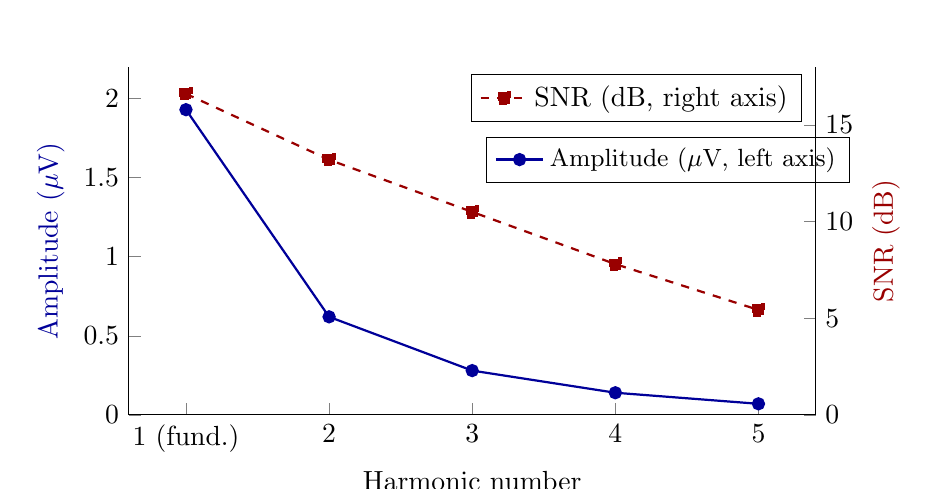
\begin{tikzpicture}
\begin{axis}[
    width=0.85\textwidth, height=6cm,
    xlabel={Harmonic number},
    ylabel={Amplitude ($\mu$V)},
    ylabel style={color=blue!60!black},
    xtick={1,2,3,4,5},
    xticklabels={1 (fund.), 2, 3, 4, 5},
    ymin=0, ymax=2.2,
    axis y line*=left,
    axis x line*=bottom,
    legend style={at={(0.785,0.8)}, anchor=north , legend columns=2, font=\small},
]
\addplot[color=blue!60!black, mark=*, thick] coordinates {
    (1, 1.93) (2, 0.62) (3, 0.28) (4, 0.14) (5, 0.07)
};
\addlegendentry{Amplitude ($\mu$V, left axis)}
\end{axis}
\begin{axis}[
    width=0.85\textwidth, height=6cm,
    ylabel={SNR (dB)},
    ylabel style={color=red!60!black},
    xtick=\empty,
    ymin=0, ymax=18,
    axis y line*=right,
    axis x line=none,
    hide x axis,
]
\addplot[color=red!60!black, mark=square*, thick, dashed] coordinates {
    (1, 16.61) (2, 13.2) (3, 10.5) (4, 7.8) (5, 5.43)
};
\addlegendentry{SNR (dB, right axis)}
\end{axis}
\end{tikzpicture}
\caption{Harmonic amplitude versus signal-to-noise ratio (SNR) for SSVEP, using the fundamental and fifth-harmonic values reported by Chen \textit{et al.}~\cite{chen2015fbcca} (endpoints exact; intermediate harmonics 2--4 interpolated for illustration, not individually reported in the source). Amplitude falls by more than an order of magnitude while SNR falls only by roughly a third, because background EEG noise decays at a comparable rate -- the resource FBCCA's filter bank, and broadband c-VEP encoding, both exploit.}
\label{fig:harmonic-snr}
\end{figure}

\subsection{The Emerging Bottleneck: Cross-Subject and Low-Calibration Robustness}

Table~\ref{tab:sota} shows a persistent gap between training-free methods and calibration-based methods; Zerafa \textit{et al.}'s pooled comparison puts this gap, averaged across the studies they surveyed, at roughly 7--46 percentage points of accuracy depending on comparison type~\cite{zerafa2018train}. Two more recent pieces of evidence sharpen this picture considerably. First, Li \textit{et al.} show a concrete, controlled instance of the problem: on the same Benchmark data set, a training-free FBCCA baseline reaches only 58.90\%~$\pm$14.51\% average accuracy, while their cross-subject transfer method SUTL raises this to 75.53\%~$\pm$12.72\% -- a real improvement, but one that leaves a substantial gap relative to the roughly 90\% accuracy reported for fully subject-specific TRCA under comparable conditions~\cite{li2024sutl,nakanishi2018trca}. Second, Li \textit{et al.} demonstrate that a naive cross-subject transfer method can perform \emph{worse} than no transfer at all: their tt-CCA baseline suffered measurable negative transfer on the BETA data set, falling below the training-free FBCCA baseline it was meant to improve on~\cite{li2024sutl}. This is qualitatively different from the noise-robustness problem in Section~3.1, where more data or a better spatial filter reliably helps; here, the wrong kind of ``help'' (poorly selected source-subject data) can actively hurt.

A related, but distinct, instance of the same underlying problem occurs \emph{within} a single subject: a decoder calibrated once, at the start of a session, is implicitly assuming that the subject's own EEG response stays stable for the rest of the session. Wong \textit{et al.} show this assumption is costly -- an online-adapting classifier that keeps updating its templates from the subject's own ongoing trials measurably outperforms a static, once-calibrated classifier~\cite{wong2022onlineadaptation}. Miao \textit{et al.}'s c-VEP results reinforce the same underlying point from a different angle: a training-free (zero-shot) linear model reached only 65.35~$\pm$31.68~bits/min, while adding just a one-minute, subject-specific calibration raised this to 90.71~$\pm$23.19~bits/min, and adding cross-subject transfer on top of that reached 250.16~bits/min~\cite{miao2024cvepminimal} -- a clear, monotonic illustration that \emph{some} calibration information, whether from the subject or from other subjects, is what closes the training-free gap. Zhang and Tao's 2026 review confirms this is recognized as a field-wide concern, and further notes that most published cross-subject methods do not report complete generalization curves under a shared protocol, which makes it difficult to compare how well different proposed solutions actually close the gap~\cite{zhang2026mobilereview}. Section~4.2 (H2) proposes online adaptation, directly following Wong \textit{et al.}~\cite{wong2022onlineadaptation}, as this project's concrete mechanism targeting this dimension.

\subsection{An Underexplored Dimension: Adversarial Robustness}

Only one paper in the reviewed set addresses robustness to deliberately adversarial input. Bian \textit{et al.} show that a simple square-wave perturbation, added to as few as four occipital channels (or even a single well-chosen channel) at just 30\% of the signal's own standard deviation, can force a training-free CCA or FBCCA classifier to output an attacker-chosen target with an attack success rate near 100\% on the Benchmark data set and roughly 90\% on the BETA data set~\cite{bian2022squarewave}. This attack survives standard band-pass preprocessing and is largely insensitive to both the perturbation's phase and the trial length used~\cite{bian2022squarewave} -- properties the authors themselves describe as making \emph{the attack} robust, a useful reminder that ``robustness'' in this literature is sometimes a property claimed by the attacker rather than the defender. Critically, the same authors found that training-based methods (extended CCA, multi-stimulus TRCA, and TRCA variants) required a much larger, and therefore more easily detectable, perturbation amplitude to attack successfully~\cite{bian2022squarewave}. Because the reported attack specifically exploits a fixed, narrowband target frequency, it also motivates a hypothesis not tested in the original paper: a broadband, pseudorandom-code stimulus (c-VEP) may resist this particular attack mechanism differently than a narrowband SSVEP stimulus does, simply because there is no single dominant frequency for a narrowband perturbation to imitate. This possibility is developed as H3 in Section~4.3; it is a hypothesis motivated by the mechanism of the attack, not a claim tested by Bian \textit{et al.} or by any paper in the current reading list.

\subsection{Comparative Summary of the Three Robustness Dimensions}

Table~\ref{tab:robustness} summarizes the argument of this section, together with the mechanism (H1, H2, or H3) that Section~4 proposes for each dimension.

\begin{table}[htbp]
\centering
\caption{Comparison of the three robustness dimensions distinguished in Section~1.3, and the mechanism this project proposes for each.}
\label{tab:robustness}
\small
\resizebox{\textwidth}{!}{%
\begin{tabular}{@{}p{2.6cm} p{4.4cm} p{4.6cm} p{4.2cm}@{}}
\toprule
\textbf{Dimension} & \textbf{Source of variability / threat} & \textbf{Maturity, on evidence reviewed} & \textbf{Proposed mechanism} \\
\midrule
Within-trial noise robustness &
Background EEG noise, limited recording time, single fixed subject &
Largely addressed by CCA $\rightarrow$ FBCCA $\rightarrow$ TRCA/TDCA $\rightarrow$ JFPTS; incremental gains continue &
\textbf{H1}: dual-modality (color+frequency) redundancy on the STOP key \\
\addlinespace
Cross-subject / low-calibration robustness (incl.\ within-subject drift) &
Inter-subject EEG variability; risk of negative transfer; within-session non-stationarity &
Emerging bottleneck; partially addressed (SUTL, minimal-calibration c-VEP, online adaptation); not fully closed &
\textbf{H2}: trial-by-trial online adaptation \\
\addlinespace
Adversarial robustness &
Deliberately crafted, typically narrowband perturbation &
Largely open; only one paper in the current reading list &
\textbf{H3} (stretch): broadband c-VEP encoding as a candidate mitigation \\
\bottomrule
\end{tabular}
}
\end{table}

\subsection{What This Implies for the Rest of the Project}

Taken together, Sections~3.1--3.4 motivate a project structure that targets all three robustness dimensions with a single, concrete, hardware-grounded platform: the five-key wheelchair control panel described in Section~6. Rather than treating the three dimensions as three separate literature-review exercises, this report proposes and tests three mechanisms -- H1, H2, and H3 -- each targeting one dimension, on the same physical device. Section~4 explains \emph{why} each mechanism is expected to help; Section~5 describes \emph{how} each will be tested; Sections~6--7 describe the hardware and a first, single-subject prototype pass toward that testing.


% =====================================================================
\section{Proposed Robustness Mechanisms: H1, H2, and H3}
% =====================================================================

This section explains why each of the three proposed mechanisms is expected to improve robustness, and along which of the three dimensions defined in Section~1.3 and summarized in Table~\ref{tab:robustness}. All three mechanisms are designed to be tested on the same physical platform: a five-key stimulus panel (Forward, Backward, Left, Right, STOP), described fully in Section~6, in which STOP is treated as the safety-critical key and therefore receives the most redundancy.

\subsection{H1: Dual-Modality Color-Plus-Frequency Redundancy on the STOP Key}

\textbf{The mechanism.} In the panel built for this project, four keys (Forward, Backward, Left, Right) are encoded by frequency alone, using single-color LEDs. The STOP key is additionally built from a distinct-colored LED cluster, so that STOP is distinguishable from the other keys by \emph{two} independent physical properties: its flicker frequency and its color.

\textbf{Why this should help.} None of the decoding methods reviewed in Section~2.2 change as a result of adding color -- color is not itself an EEG feature, and the classifier still identifies the correct key using the same frequency-recognition methods (CCA, FBCCA, and so on). The expected benefit is therefore not a change in the statistical decoding step, but a change in the input to that step: a visually distinct STOP key is easier and faster for the subject to locate and fixate on, particularly under time pressure or partial visual impairment, which is directly relevant to the wheelchair-control application this panel is designed for~\cite{nicolasalonso2012bci}. A faster, more confident fixation is expected to produce a cleaner, higher-SNR SSVEP response at the target frequency, which benefits every decoding method in Table~\ref{tab:pipeline-taxonomy} without requiring any of them to be modified. This reasoning is an extension of a general engineering principle -- that redundant, independently-verifiable coding improves the reliability of a communication channel -- applied here at the level of stimulus design rather than at the level of the decoding algorithm. No paper in the current reading list tests this specific combination for SSVEP-BCI; H1 is accordingly this project's own proposed contribution, not a replication of an existing result.

\textbf{Target dimension.} H1 targets dimension (a), within-trial noise/reliability robustness, and specifically the safety-critical STOP command, where a missed or delayed classification has the highest real-world cost of any of the five keys.

\subsection{H2: Trial-by-Trial Online Adaptation}

\textbf{The mechanism.} Rather than calibrating each key's spatial-temporal template once, at the start of a session, and then holding it fixed, an online-adaptive classifier updates each key's template after every trial the system believes it classified correctly, blending the new trial's data into the existing template with a small update weight.

\textbf{Why this should help.} Section~3.2 established that EEG is non-stationary within a session, because of fatigue, attention fluctuation, and gradual changes in electrode contact quality~\cite{nicolasalonso2012bci}. A classifier calibrated only once at the start of a session is implicitly assuming this does not happen. Wong \textit{et al.} directly test the alternative and find that online adaptation measurably improves SSVEP-BCI performance relative to a static classifier~\cite{wong2022onlineadaptation}; this project's H2 mechanism is a direct application of the same principle to the five-key wheelchair panel described in Section~6, which -- to the best of this review's knowledge -- has not previously been tested for this specific combination of stimulus layout and command set.

\textbf{Target dimension.} H2 targets dimension (b), specifically its within-subject, temporal-drift form: robustness to the subject's \emph{own} signal changing over the course of a single session, as distinct from the between-subject transfer problem addressed by methods such as SUTL~\cite{li2024sutl}.

\subsection{H3 (Stretch Goal): A Code-Modulated (c-VEP) STOP Key}

\textbf{The mechanism.} As an additional, higher-effort test, the STOP key's frequency-based flicker can be replaced by a code-modulated (c-VEP) stimulus: instead of flickering at a fixed 10~Hz, the LED cluster is switched on and off according to a pseudorandom binary sequence (an m-sequence), and the classifier identifies the correct key by finding which time-shift of the reference sequence best matches the recorded EEG. This design directly follows Sun \textit{et al.}'s cyclic-shift c-VEP approach~\cite{sun2022cyclicshift} and is implemented in this project's own firmware (Section~6).

\textbf{Why this should help.} Two independent lines of reasoning motivate H3, targeting two different robustness dimensions:
\begin{itemize}
  \item \emph{Calibration efficiency (dimension b).} Miao \textit{et al.} show that a c-VEP system, historically assumed to need extensive per-subject calibration, can reach SSVEP-comparable performance (250.16~bits/min) with only about one minute of calibration data, once a suitable spatial-temporal pattern estimation method is used~\cite{miao2024cvepminimal}. If this holds on this project's own hardware, c-VEP would offer competitive performance without adding meaningfully to the calibration burden that H2 is already designed to reduce.
  \item \emph{Adversarial resistance (dimension c, speculative).} Bian \textit{et al.}'s square-wave attack specifically exploits a fixed, narrowband target frequency~\cite{bian2022squarewave}. Because a pseudorandom c-VEP code spreads its energy across a broad frequency range rather than concentrating it at one frequency, it is plausible -- though not tested by any paper in the current reading list, and not yet tested by this project either -- that a c-VEP-coded STOP key would be harder to spoof with the same narrowband attack mechanism. This is stated here explicitly as an untested hypothesis, not a validated robustness claim.
\end{itemize}

\textbf{Target dimension.} H3 targets dimension (b) directly (via minimal-calibration performance) and dimension (c) speculatively (via broadband robustness to narrowband adversarial perturbation). It is marked a ``stretch goal'' because, as reported in Section~7, a prototype attempt at c-VEP decoding on this project's own hardware did not yet succeed, for reasons diagnosed in Section~7.3.

\subsection{Summary}

Table~\ref{tab:h123-summary} restates the three mechanisms, their target dimensions, and their evidentiary status at the time of writing.

\begin{table}[htbp]
\centering
\caption{Summary of the three proposed mechanisms.}
\label{tab:h123-summary}
\small
\begin{tabular}{@{}p{1.0cm} p{4.5cm} p{2.6cm} p{4.1cm}@{}}
\toprule
\textbf{ID} & \textbf{Mechanism} & \textbf{Target dimension(s)} & \textbf{Status at time of writing} \\
\midrule
H1 & Color+frequency redundancy on STOP & (a) noise/reliability & Hardware built; not yet tested (Section~8) \\
H2 & Trial-by-trial online adaptation & (b) within-subject drift & Protocol designed (Section~5.3); not yet tested \\
H3 & c-VEP STOP key & (b) calibration efficiency; (c) adversarial (speculative) & Hardware and firmware built; first decoding attempt unsuccessful (Section~7.3); diagnosed, not yet resolved \\
\bottomrule
\end{tabular}
\end{table}


% =====================================================================
\section{Experimental Protocol for Testing H1, H2, and H3}
% =====================================================================

This section summarizes the experimental protocol designed to test H1--H3. It is presented here at the level of detail typical of a Methods section; a more detailed step-by-step protocol document, including the full Python analysis pipeline, exists as separate project material.

\subsection{General Session Structure and Synchronization}

Following the two-stage design used by Miao \textit{et al.}~\cite{miao2024cvepminimal}, each planned session is structured as (i) a short, single-target calibration stage, in which each key is presented alone and repeated several times, followed by (ii) a multi-key identification stage, in which all relevant keys are presented together and the subject is cued to fixate on a specific one per trial. Precise trial timing (stimulation duration, inter-trial interval, and number of repetitions per key) follows the parameters summarized in Table~\ref{tab:trial-params}.

\begin{table}[htbp]
\centering
\caption{Planned trial parameters for H1--H3 testing, following Miao \textit{et al.}~\cite{miao2024cvepminimal} and Chen \textit{et al.}~\cite{chen2015pnas}.}
\label{tab:trial-params}
\small
\begin{tabular}{@{}p{6.2cm} p{2.5cm} p{4.6cm}@{}}
\toprule
\textbf{Parameter} & \textbf{Value} & \textbf{Rationale} \\
\midrule
Calibration trial duration & 3~s & Matches~\cite{miao2024cvepminimal} \\
Calibration repetitions per key & 4 trials & Matches~\cite{miao2024cvepminimal} \\
Multi-key trial: gaze-shift + stimulation & 0.5~s + 2--3~s & Matches ITR convention in~\cite{chen2015pnas} \\
Blocks per condition & 5 blocks $\times$ 5 trials (one per key, randomized order) & Matches online FBCCA protocol in~\cite{chen2015fbcca} \\
\bottomrule
\end{tabular}
\end{table}

A hardware synchronization marker, sent from the panel's microcontroller to the recording computer at the exact onset of each trial, is required for precise epoch labeling; this marker is not yet implemented in firmware (see Section~8).

\subsection{H1 Protocol: Color+Frequency Redundancy}

Two blocks are run on the STOP key only, holding the decoding method fixed: one block with STOP encoded by frequency alone (matching the other four keys' encoding style), and one block with STOP encoded by both frequency and its distinct color. Classification accuracy and information transfer rate (ITR) are compared between the two blocks using the same trial count and the same classifier, so that any difference can be attributed to the stimulus change rather than to the decoding algorithm.

\subsection{H2 Protocol: Static versus Adaptive Classifier}

Two multi-key identification blocks are run under otherwise identical conditions: one using a static classifier (calibrated once, held fixed for the whole block), and one using an online-adaptive classifier that updates each key's template after every trial it believes was classified correctly, following the update rule used by Wong \textit{et al.}~\cite{wong2022onlineadaptation}. Accuracy is compared both as a single pooled number and per block, since a declining or rising trend across blocks is itself diagnostic evidence for or against the presence of within-session drift.

\subsection{H3 Protocol: SSVEP-STOP versus c-VEP-STOP}

Two blocks are run on the STOP key only: one using the standard 10~Hz frequency-coded stimulus, and one using the c-VEP pseudorandom-code stimulus described in Section~6. Both blocks use the same trial count and duration; classification accuracy and ITR are compared directly, and, where feasible, robustness to injected narrowband noise is compared between the two encodings as a first, exploratory test of the adversarial-robustness hypothesis in Section~4.3.

\subsection{Statistical Analysis Plan}

For each comparison (H1, H2, H3), the plan is to report: mean accuracy $\pm$ standard deviation per condition; ITR in bits/min, computed following the formula used by Miao \textit{et al.}~\cite{miao2024cvepminimal}; a paired statistical test (McNemar's test for paired binary classification outcomes) between the two conditions being compared; and an explicit statement of sample-size limitations. As discussed in Section~8, the single-subject prototype data set described in Section~7 does not yet support this full analysis plan; it is presented here as the protocol for the data collection that remains to be carried out.


% =====================================================================
\section{Control Panel Assembly}
% =====================================================================

\subsection{Overview}

The stimulus panel is a physical, five-key device corresponding to the five wheelchair commands: Forward, Backward, Left, Right, and STOP. It is built around an STM32F103C8T6 (``Blue Pill'') microcontroller, which drives all five LED clusters using hardware timer interrupts, in both a frequency-coded (SSVEP) mode and a pseudorandom-code (c-VEP) mode, selectable in firmware.

\subsection{Required Tools and Components}

\begin{itemize}
  \item STM32F103C8T6 ``Blue Pill'' development board, and an ST-Link programmer/debugger.
  \item ULN2003AG Darlington transistor array, used to drive each LED cluster safely above the microcontroller's per-pin current limit.
  \item 17 white ``Hyperlight'' 5~mm LEDs (V $=$ 3--3.2~V, I $=$ 15--20~mA): 3 per side key (Forward, Backward, Left, Right) and 5 for the STOP key.
  \item Current-limiting resistors, approximately 100--120~$\Omega$ per LED (calculated from a 5~V supply rail).
  \item A photoresistor, used with a spare analog-to-digital converter (ADC) input to verify the true LED flicker frequency against the value programmed in firmware.
  \item An HC-05 Bluetooth module, intended for sending a trial-synchronization marker to the recording computer (not yet implemented in firmware; see Section~8).
  \item Power supply chain: an XL6009E1 boost converter feeding an L7805CV linear regulator, providing a clean 5~V rail to the Blue Pill and LED circuits.
  \item Semi-transparent diffuser material (e.g.\ tracing paper or frosted acrylic) over each LED cluster, for even light distribution.
  \item General assembly tools: breadboard or perfboard, soldering iron, multimeter, and an oscilloscope or logic analyzer for verifying timer-generated flicker frequencies before use with a human subject.
\end{itemize}

\subsection{Practical Setup}

The panel base is a 10~cm~$\times$~10~cm rectangular board. Four rectangular side keys (4~cm~$\times$~1.8~cm) are placed with a 0.2~cm margin from the panel border, arranged in a ``plus/D-pad'' layout matching the physical direction of the corresponding wheelchair command; a 3~cm~$\times$~3~cm STOP key is centered on the panel. Each STM32 timer/GPIO output drives one ULN2003AG channel, which in turn drives one key's LED cluster (in parallel, each LED with its own current-limiting resistor). In SSVEP mode, the five keys flicker at fixed frequencies (Forward 12~Hz, Backward 8~Hz, Left 13~Hz, Right 9~Hz, STOP 10~Hz), generated by hardware timer interrupts (TIM2 and TIM3) to avoid the frequency jitter that a software delay loop would introduce. In c-VEP mode, all five keys are driven from the same 127-bit maximal-length sequence (m-sequence), generated by a 7-bit linear feedback shift register (LFSR, primitive polynomial $x^7+x^6+1$) updated at approximately 60~Hz, with each key assigned a different cyclic shift of the sequence (Forward 0, Backward 25, Left 50, Right 75, STOP 100 chips), following the design principle demonstrated by Sun \textit{et al.}~\cite{sun2022cyclicshift}. Figure~\ref{fig:dpad-geometry} shows this layout to scale, with the verified clearances between keys.

\begin{figure}[htbp]
\centering
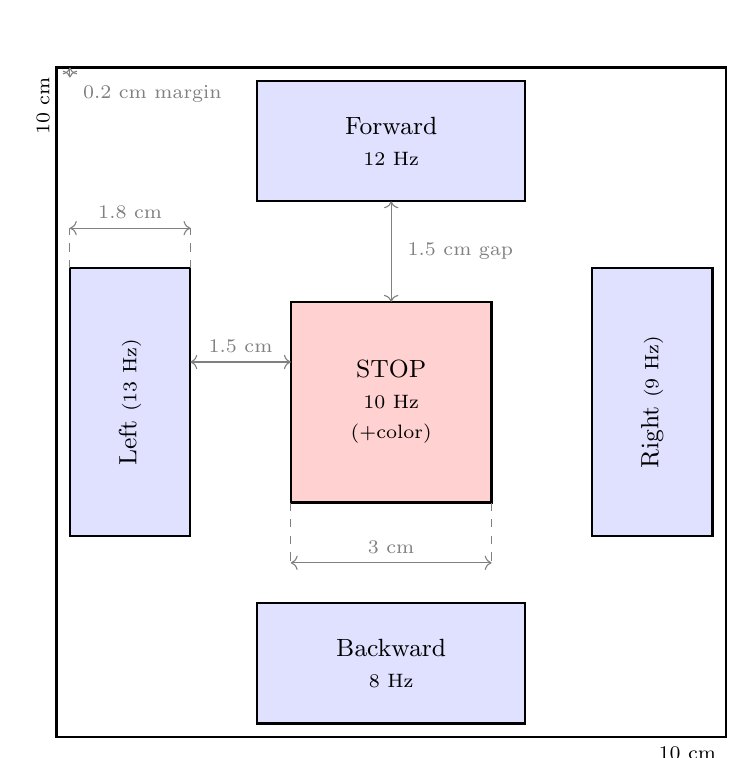
\begin{tikzpicture}[scale=0.85, every node/.style={font=\small, align=center}]
  % Panel border
  \draw[thick] (0,0) rectangle (10,10);
  \node[below left, font=\scriptsize] at (10,0) {10~cm};
  \node[left, font=\scriptsize, rotate=90] at (-0.2,10) {10~cm};

  % Forward (top)
  \draw[fill=blue!12, thick] (3,8) rectangle (7,9.8);
  \node at (5,8.9) {Forward \\ \scriptsize 12~Hz};

  % Backward (bottom)
  \draw[fill=blue!12, thick] (3,0.2) rectangle (7,2.0);
  \node at (5,1.1) {Backward \\ \scriptsize 8~Hz};

  % Left
  \draw[fill=blue!12, thick] (0.2,3) rectangle (2.0,7);
  \node[rotate=90] at (1.1,5) {Left \scriptsize (13~Hz)};

  % Right
  \draw[fill=blue!12, thick] (8.0,3) rectangle (9.8,7);
  \node[rotate=90] at (8.9,5) {Right \scriptsize (9~Hz)};

  % STOP (center, distinct color)
  \draw[fill=red!18, thick] (3.5,3.5) rectangle (6.5,6.5);
  \node at (5,5) {STOP \\ \scriptsize 10~Hz \\ \scriptsize (+color)};

  % Clearance annotations
  \draw[<->, gray] (5,6.5) -- (5,8.0);
  \node[right, gray, font=\scriptsize] at (5.1,7.25) {1.5~cm gap};
  \draw[<->, gray] (2.0,5.6) -- (3.5,5.6);
  \node[above, gray, font=\scriptsize] at (2.75,5.6) {1.5~cm};
  \draw[<->, gray] (0.2,7.6) -- (2,7.6);
  \draw[dashed, gray] (0.2,7) -- (0.2,7.6);
  \draw[dashed, gray] (2,7) -- (2,7.6);
  \node[above, gray, font=\scriptsize] at (1.1,7.6) {1.8~cm};

    \draw[<->, gray] (3.5,2.6) -- (6.5,2.6);
  \draw[dashed, gray] (3.5,3.5) -- (3.5,2.6);
  \draw[dashed, gray] (6.5,3.5) -- (6.5,2.6);
  \node[above, gray, font=\scriptsize] at (5,2.6) {3~cm};
  % Margin annotation
  \draw[<->, gray] (0.2,9.85) -- (0.2,10);
  \node[right, gray, font=\scriptsize] at (0.25, 9.6) {0.2~cm margin};
\end{tikzpicture}
\caption{To-scale layout of the five-key D-pad stimulus panel (top-down view), showing key dimensions, panel-border margins (0.2~cm), and verified inter-key clearances (1.0--1.5~cm). STOP is additionally distinguished by a distinct LED color, implementing the H1 mechanism (Section~4.1).}
\label{fig:dpad-geometry}
\end{figure}

\begin{figure}[htbp]
\centering
\includegraphics[width=\textwidth]{assembeled tool.jpg}
\caption{Physical layout of the five-key stimulus panel (placeholder).}
\label{fig:panel-photo}
\end{figure}

\begin{figure}[htbp]
\centering
\includegraphics[width=0.9\textwidth]{SSVEP_Panel (1).png}
\caption{Circuit schematic of the stimulus panel (placeholder).}
\label{fig:panel-schematic}
\end{figure}


% =====================================================================
\section{Data Generation and Analysis}
% =====================================================================

\subsection{Data Generation for One Subject}

A first, prototype data-collection pass was carried out with a single subject (male, age 61), recorded to separate European Data Format (.edf) files per trial, using five parts:

\begin{enumerate}
  \item \textbf{Baseline.} Eyes-open and eyes-closed resting recordings, 7 minutes each, with no stimulus, used to confirm basic signal quality (e.g.\ the expected increase in occipital alpha-band power during eyes-closed rest).
  \item \textbf{SSVEP single-key.} Each of the five keys flickered alone; the subject fixated on it for 10~s per trial, 5 trials per key.
  \item \textbf{SSVEP multi-key.} All five keys flickered simultaneously, each at its own frequency; the subject was cued to fixate on one of three keys (Backward, Left, STOP) per 10~s trial.
  \item \textbf{c-VEP single-key.} Identical structure to Part~2, using the c-VEP stimulus described in Section~6.2 in place of fixed-frequency flicker.
  \item \textbf{c-VEP multi-key.} Identical structure to Part~3, using the c-VEP stimulus in place of fixed-frequency flicker.
\end{enumerate}

\subsection{Mismatch With the Intended Protocol}

This data set deviates from the protocol described in Section~5 in two respects, both stated here explicitly rather than left implicit. First, no hardware synchronization marker was used: for each trial, the panel was switched on, recording began, and the subject was told verbally, approximately one second later, which key to fixate on. Second, the multi-key conditions (Parts 3 and 5) tested only three of the five keys (Backward, Left, STOP), not all five. To compensate for the missing hardware marker, a fixed discard-and-analysis window was applied uniformly to every 10~s trial: the first 2.0~s are discarded (covering the verbal-cue delay, the subject's reaction time, and the SSVEP/c-VEP onset transient), the following 7.5~s (2.0--9.5~s) are used for analysis, and the final 0.5~s are discarded (to avoid end-of-trial anticipation effects). This adaptation is a wider-margin version of the fixed gaze-shift discard window already used in the literature reviewed in Section~2 (e.g.\ the 0.5~s gaze-shift convention built into the ITR formula in~\cite{chen2015pnas}), rather than an ad hoc correction. Because of both deviations, this data set is treated throughout this report as a \textbf{feasibility prototype}, not as the final validation data set for H1--H3; see Section~8 for what remains before such validation is possible.

\subsection{Analysis Pipeline and Results Summary}

The prototype recordings were analyzed in Python (documented in the accompanying notebook, \texttt{SSVEP\_cVEP\_Analysis.ipynb}), following a bandpass-and-notch preprocessing step consistent with standard SSVEP practice, then epoched using the discard-and-analysis window described above.

For the SSVEP data (Parts 2--3), three decoding approaches of increasing sophistication were implemented and compared: a naive baseline that selects the candidate frequency with the largest single FFT peak; an improved baseline that sums FFT power across a frequency's first few harmonics before selecting the maximum; and a full CCA/FBCCA-style correlation classifier using sine/cosine reference signals at each candidate frequency and its harmonics, following the method in~\cite{lin2007cca,chen2015fbcca}. Classification accuracy improved substantially and consistently across this progression, in the direction predicted by Section~2.2's literature review (naive FFT peak-picking performing worst, harmonic-aware summation performing better, and full CCA/FBCCA-style correlation performing best) -- see Figure~\ref{fig:ssvep-progression}.

For the c-VEP data (Parts 4--5), a lag-correlation classifier was implemented: the recorded EEG is correlated against the reference m-sequence at every candidate cyclic shift, and the shift with the highest correlation is selected, following the general principle used by Miao \textit{et al.}~\cite{miao2024cvepminimal}. This classifier did not achieve better-than-chance classification accuracy on the prototype data set. The diagnosed reason is methodologically important and connects directly back to Section~3.2's argument: a simple, training-free lag-correlation classifier implicitly assumes that the recorded EEG is a close copy of the stimulus code's own shape, whereas the true relationship between a broadband code and the resulting EEG response is a smoothed, subject-specific temporal response function (TRF) that must be estimated from calibration data before decoding can work, exactly as Miao \textit{et al.} and Liu \textit{et al.}'s TDCA formulation make explicit~\cite{miao2024cvepminimal,liu2021tdca}. In other words, \textbf{this project's own empirical failure independently reproduces the same training-free/calibration-based tension identified in Section~3.2 of the literature review}, using a completely different method (a hardware prototype and a simple correlation classifier) than the papers that first identified it. This is presented here as a genuine, if negative, finding: c-VEP decoding on this hardware will require implementing a calibration-based approach (TDCA, or the linear-modeling method of~\cite{miao2024cvepminimal}) before H3 can be properly tested, rather than being usable ``out of the box'' with a training-free classifier the way SSVEP was.

\subsection{Most Significant Figures}

\begin{figure}[htbp]
\centering
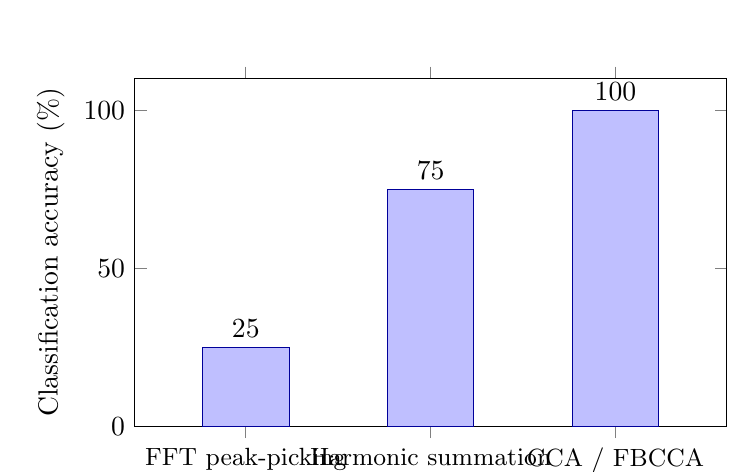
\begin{tikzpicture}
\begin{axis}[
    ybar, bar width=1.1cm,
    width=0.75\textwidth, height=6cm,
    ymin=0, ymax=110,
    ylabel={Classification accuracy (\%)},
    symbolic x coords={FFT peak-picking, Harmonic summation, CCA / FBCCA},
    xtick=data,
    x tick label style={font=\small},
    nodes near coords,
    nodes near coords align={vertical},
    enlarge x limits=0.3,
    axis line style={draw=black},
]
\addplot[fill=blue!25, draw=blue!60!black] coordinates {
    (FFT peak-picking, 25)
    (Harmonic summation, 75)
    (CCA / FBCCA, 100)
};
\end{axis}
\end{tikzpicture}
\caption{SSVEP single-key classification accuracy by decoding method, single-subject prototype data set ($N=1$, 5 trials per key). Reconstructed from the accuracy values reported in \texttt{SSVEP\_cVEP\_Analysis}. \textbf{Verify exact percentages against the notebook's current output before final submission.} The upward trend (naive FFT $\rightarrow$ harmonic-aware $\rightarrow$ correlation-based) matches the pattern predicted by the literature reviewed in Section~2.2.}
\label{fig:ssvep-progression}
\end{figure}

\begin{figure}[htbp]
\centering
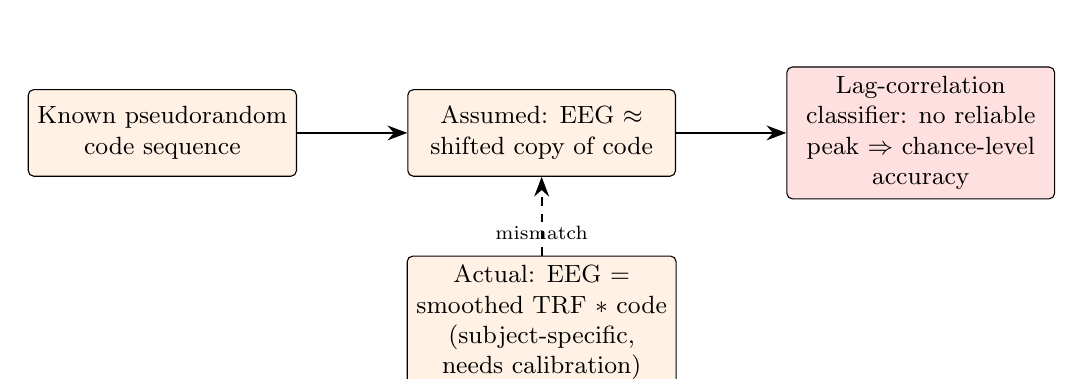
\begin{tikzpicture}[
  every node/.style={font=\small},
  stage/.style={draw, rounded corners=2pt, minimum width=3.4cm, minimum height=1.1cm, align=center, fill=orange!10},
  arr/.style={-{Stealth[length=2.5mm]}, thick}
]
  \node[stage] (code) {Known pseudorandom\\code sequence};
  \node[stage, right=1.4cm of code] (naive) {Assumed: EEG $\approx$\\shifted copy of code};
  \node[stage, below=1.0cm of naive] (real) {Actual: EEG $=$\\smoothed TRF $*$ code\\(subject-specific,\\needs calibration)};
  \node[stage, right=1.4cm of naive, fill=red!12] (fail) {Lag-correlation\\classifier: no reliable\\peak $\Rightarrow$ chance-level\\accuracy};

  \draw[arr] (code) -- (naive);
  \draw[arr] (naive) -- (fail);
  \draw[arr, dashed] (real) -- (naive) node[midway, below, font=\scriptsize] {mismatch};
\end{tikzpicture}
\caption{Conceptual diagram of the diagnosed c-VEP decoding failure. This is an explanatory illustration of the mechanism described in Section~7.3, \textbf{not a plot of recorded experimental data}; it should be replaced with the actual lag-correlation plot exported from \texttt{SSVEP\_cVEP\_Analysis.ipynb} once available.}
\label{fig:cvep-failure}
\end{figure}

\begin{figure}[htbp]
\centering
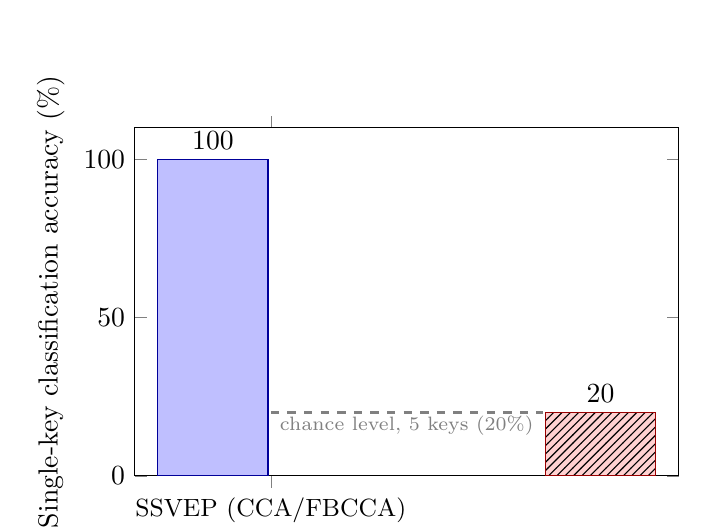
\begin{tikzpicture}
\begin{axis}[
    ybar, bar width=1.4cm,
    width=0.7\textwidth, height=6cm,
    ymin=0, ymax=110,
    ylabel={Single-key classification accuracy (\%)},
    symbolic x coords={SSVEP, cVEP},
    xtick=data,
    xticklabels={SSVEP (CCA/FBCCA), c-VEP (lag-correlation)},
    x tick label style={font=\small, align=center},
    nodes near coords,
    enlarge x limits=0.5,
    axis line style={draw=black},
]
\addplot[fill=blue!25, draw=blue!60!black] coordinates {
    (SSVEP, 100)
};
\addplot[fill=red!18, draw=red!60!black, postaction={pattern=north east lines}] coordinates {
    (cVEP, 20)
};
\draw[dashed, thick, gray] (axis cs:SSVEP,20) -- (axis cs:cVEP,20)
    node[midway, below, font=\scriptsize, fill=white, inner sep=1pt] {chance level, 5 keys (20\%)};
\end{axis}
\end{tikzpicture}
\caption{Single-key classification accuracy, SSVEP versus c-VEP, single-subject prototype data set ($N=1$). The c-VEP bar is drawn \textbf{at the chance-level reference line (20\%, five equiprobable keys)} because the lag-correlation classifier did not achieve better-than-chance accuracy (Section~7.3); it is \textbf{not} a fabricated precise measurement, and should be replaced with the true measured value once re-verified against \texttt{SSVEP\_cVEP\_Analysis.ipynb}. The gap illustrates the calibration-based decoding this project still needs to implement (Section~8.2).}
\label{fig:ssvep-vs-cvep}
\end{figure}


% =====================================================================
\section{Accomplished and Remaining Work}
% =====================================================================

\subsection{Accomplished}

\begin{itemize}
  \item A literature review of approximately 20 papers, organized by the pipeline-stage $\times$ training-taxonomy framework (Section~2.1) and synthesized into a three-dimensional robustness taxonomy (Section~3).
  \item Selection and justification of three concrete robustness mechanisms, H1--H3, each targeting a specific dimension of that taxonomy (Section~4).
  \item Design of a full experimental protocol for testing H1--H3 (Section~5).
  \item Physical construction of a five-key SSVEP/c-VEP stimulus panel, with STM32 firmware implementing both frequency-coded and pseudorandom-code-modulated stimulation (Section~6).
  \item A first, single-subject prototype EEG recording pass (five parts, Section~7.1) and a working Python analysis pipeline, including a validated SSVEP decoding chain (FFT peak-picking $\rightarrow$ harmonic summation $\rightarrow$ CCA/FBCCA) and a first c-VEP decoding attempt (Section~7.3).
  \item A diagnosed, literature-consistent explanation for why the first c-VEP decoding attempt did not succeed, directly connecting the project's own empirical result back to the calibration-robustness argument of Section~3.2.
  \item A complete, verified bibliography covering all references used across the literature review and the H1--H3 proposal.
\end{itemize}

\subsection{Remaining}

\begin{itemize}
  \item \textbf{Hardware synchronization.} A trial-start marker (e.g.\ over the existing HC-05 Bluetooth link) has not yet been added to the firmware; without it, future recordings will face the same manual-timing limitation as the current prototype.
  \item \textbf{Validation data set.} No further data collection is currently planned in the near term; the single-subject prototype described in Section~7 is the only data set available at the time of writing, and it is explicitly not sufficient to test H1, H2, or H3 (it was not designed to isolate these comparisons, and lacks the redundant-STOP, adaptive-classifier, and SSVEP-vs-c-VEP-STOP conditions specified in Section~5). Testing H1--H3 properly therefore remains future work, to be carried out once further recording sessions become possible.
  \item \textbf{c-VEP calibration-based decoding.} The training-free lag-correlation classifier used in Section~7.3 is not expected to work; a calibration-based approach (TDCA, following~\cite{liu2021tdca}, or the linear-modeling method of~\cite{miao2024cvepminimal}) has not yet been implemented.
  \item \textbf{m-sequence orthogonality verification.} The five cyclic shifts used in the firmware's c-VEP mode (Section~6.2) have not yet been formally verified, in software, to be sufficiently distinguishable from one another under the project's actual trial length and sampling rate.
  \item \textbf{Physical and schematic figures.} Figures~\ref{fig:panel-photo} and~\ref{fig:panel-schematic} remain placeholders pending photography and schematic capture of the assembled hardware.
  \item \textbf{GitHub repository.} A public repository for the project's code, firmware, and (where appropriate) data has not yet been created; see the placeholder link in Section~9.
\end{itemize}

\subsection{Expectations}

Based on the reasoning in Section~4 and the general pattern already observed in the SSVEP decoding results (Section~7.3, Figure~\ref{fig:ssvep-progression}), the following outcomes are expected, but are explicitly stated as \emph{expectations}, not results, since none of H1--H3 has yet been tested under the protocol of Section~5:

\begin{itemize}
  \item \textbf{H1} is expected to show a modest but measurable improvement in STOP-key classification accuracy and/or reaction time when color redundancy is present, consistent with the reliability-of-fixation reasoning in Section~4.1; the effect is expected to be small relative to decoding-algorithm differences, since it operates upstream of the classifier.
  \item \textbf{H2} is expected to show an accuracy or ITR trend that improves, or at least does not degrade, across blocks under the adaptive classifier relative to the static one, particularly in longer sessions where within-session drift has more time to manifest; a null or negative result would itself be informative, given the risk of adaptation reinforcing its own errors discussed when this mechanism was first designed.
  \item \textbf{H3} is expected to remain infeasible with a training-free classifier, consistent with Section~7.3's diagnosis, until a calibration-based decoder (TDCA or linear modeling) is implemented; once implemented, performance comparable to SSVEP is plausible given Miao \textit{et al.}'s results under similarly minimal calibration~\cite{miao2024cvepminimal}, but this has not yet been tested on this project's own hardware and subject pool.
\end{itemize}


% =====================================================================
\section{Conclusion}
% =====================================================================

This report has reviewed the SSVEP-BCI decoding literature through the lens of a three-dimensional robustness taxonomy (within-trial noise, cross-subject/low-calibration, and adversarial robustness), and has used that taxonomy to motivate three concrete, testable robustness mechanisms -- dual-modality redundancy on a safety-critical command (H1), trial-by-trial online adaptation (H2), and an alternative broadband stimulus encoding (H3) -- implemented on a purpose-built five-key wheelchair control panel. A first, single-subject hardware and software prototype has validated the feasibility of the panel and the SSVEP decoding pipeline, and has produced a diagnosed, literature-consistent negative result for training-free c-VEP decoding that directly reinforces this report's own central argument about the role of calibration in robustness. The project's next concrete step is the synchronized, multi-condition data collection specified in Section~5, which remains the primary blocker between the current prototype and a genuine empirical test of H1--H3.



\\
\\
All code, firmware, and supporting materials for this project are maintained at:\\
$$\boxed{
\text{
\url{https://github.com/farouoq83/ssvep-robust-bci}}}
$$
% =====================================================================
\bibliographystyle{IEEEtran}
\bibliography{refs}


\end{document}